%%%%%%%%%%%%%%%%%%%%%%%%%%%%%%%%%%%%%%%%%%%%%%%%%%%%%%%%%%%%%%%%%%%%%%%%%%%%%%%%
%2345678901234567890123456789012345678901234567890123456789012345678901234567890
%        1         2         3         4         5         6         7         8

\documentclass[letterpaper, 10 pt, conference]{ieeeconf}  % Comment this line out
                                                          % if you need a4paper
%\documentclass[a4paper, 10pt, conference]{ieeeconf}      % Use this line for a4
                                                          % paper

\IEEEoverridecommandlockouts                              % This command is only
                                                          % needed if you want to
                                                          % use the \thanks command
\overrideIEEEmargins
% See the \addtolength command later in the file to balance the column lengths
% on the last page of the document

\usepackage[utf8]{inputenc}
\usepackage[T1]{fontenc}
\usepackage[english]{babel}
\usepackage{graphicx}

% The following packages can be found on http:\\www.ctan.org
% \usepackage{graphics} % for pdf, bitmapped graphics files
%\usepackage{epsfig} % for postscript graphics files
%\usepackage{mathptmx} % assumes new font selection scheme installed
%\usepackage{mathptmx} % assumes new font selection scheme installed
%\usepackage{amsmath} % assumes amsmath package installed
%\usepackage{amssymb}  % assumes amsmath package installed

\title{\LARGE \bf
Design of a Public Protection and Disaster Relief Network for São Miguel Island}

\author{ \parbox{3 in}{\centering Daniel Rebelo\\
        % \thanks{*Use the $\backslash$thanks command to put information here}\\
        Instituto Superior Técnico / Instituto de Telecomunicações\\
        University of Lisbon\\
        Lisbon, Portugal\\
        {\tt\small danielrebelo@tecnico.ulisboa.pt}}
        \hspace*{ 0.5 in}
        \parbox{3 in}{ \centering António L. Topa\\
        %\thanks{**The footnote marks may be inserted manually}\\
        Instituto Superior Técnico / Instituto de Telecomunicações\\
        University of Lisbon\\
        Lisbon, Portugal\\
        {\tt\small antonio.topa@lx.it.pt}}
}

% \author{Daniel Rebelo% <-this % stops a space
% \thanks{*This work was not supported by any organization}% <-this % stops a space
% \thanks{$^{1}$H. Kwakernaak is with Faculty of Electrical Engineering, Mathematics and Computer Science,
%         University of Twente, 7500 AE Enschede, The Netherlands
%         {\tt\small h.kwakernaak at papercept.net}}%
% \thanks{$^{2}$P. Misra is with the Department of Electrical Engineering, Wright State University,
%         Dayton, OH 45435, USA
%         {\tt\small p.misra at ieee.org}}%
% }


\begin{document}



\maketitle
\thispagestyle{empty}
\pagestyle{empty}


%%%%%%%%%%%%%%%%%%%%%%%%%%%%%%%%%%%%%%%%%%%%%%%%%%%%%%%%%%%%%%%%%%%%%%%%%%%%%%%%
\begin{abstract}
This Dissertation aims at a project of a TETRA emergency and public safety network for São Miguel Island. In the Azores, there are numerous situations of risk to people and goods every year. The damage caused by these events is partly aggravated by human occupation in areas of high sensitivity and fragility. These factors, as well as recent events in Pedrogão Grande, aroused interest in developing a project on this topic. The objective of this Dissertation is to reach mobile network coverage values greater than or equal to 95\% and reach at least 98\% of the population. For this, the use of TETRA technology is used.\par\noindent
During this Dissertation are presented the two systems implemented in the Autonomous Region of the Azores. These systems are RITERAA and SIRESP.\par\noindent
During implementation of a mobile network, for coverage and interference reasons, it is necessary to estimate the signal transmitted by the base station. Signal estimation involves the calculation of an average value and the oscillations around this value. To estimate the signal, the Okumura-Hata model and the Walfisch-Ikegami model were used.\par\noindent
The fundamental concepts of mobile networks were discussed, followed by the project implementation. Finally, simulations were performed from the values  obtained in the project sizing. It was concluded that it is possible to exceed the objectives initially set since the coverage exceeds 96\% of the study area and reaches at least 99\% of the population.
\end{abstract}


%%%%%%%%%%%%%%%%%%%%%%%%%%%%%%%%%%%%%%%%%%%%%%%%%%%%%%%%%%%%%%%%%%%%%%%%%%%%%%%%
\section{INTRODUCTION}
\noindent In the Azores are known numerous situations of risk to people and goods, the consequences of these occurrences are magnified by human occupation in areas of high sensitivity and fragility.
Every year many natural disasters victimize people and cause harm around the world. In the case of the Azores archipelago, it is the floods, slope movements, earthquakes and natural hazards that register the highest number of occurrences, causing high material damage and, in extreme situations, fatalities. \par \noindent
The small size of the islands, the volcanic nature that determines the geomorphology and geology, are factors that should be considered. In situations of heavy rainfall, devastating flooding may occur, especially in urban areas located near the streams. 
Due to the characteristics that these types of calamities usually present, it is difficult to make their prediction, creating the need for an effective emergency communication system. \par \noindent
Thus, the opportunity arose to carry out a project of an emergency and safety communications network designed explicitly for the São Miguel Island of the Eastern Group of the Azores.\par\noindent
These networks have certain factors that must be considered. In commercial networks, those factors are negligible. The interest in these networks was sparked after the recent tragedy in Pedrogão Grande, in which SIRESP played a key role. Recently, emergency and public safety networks had a crucial role in the passage of Hurricane Lorenzo through the Archipelago of the Azores.\par\noindent
This paper elaborates on a Public Protection and Disaster Relief Network for São Miguel Island. This network is developed through TETRA technology, being necessary to consider the particularities of these systems.\par\noindent
In addition to mobile coverage planning, this paper also establishes the transport network. The transport network interconnects all the base stations of this network, enabling communications with any user, the transport network will use microwave links to interconnect the base stations. \par\noindent
This network will have to overcome the difficulties provided by the island (large water surfaces on the island, extremely irregular orography).
\begin{figure}[h]
    \centering
    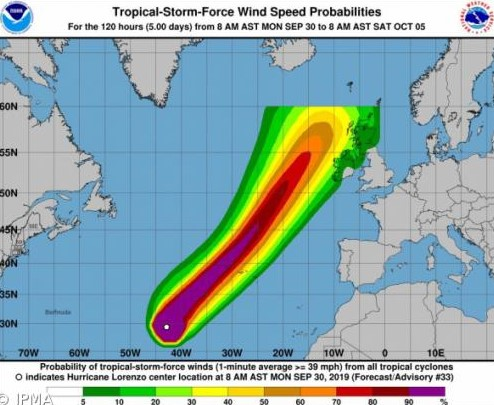
\includegraphics[width=0.4\textwidth]{Lorenzo.jpg}
    \caption{Hurricane Lorenzo}
    \label{fig:lorenzo}
\end{figure}

%%%%%%%%%%%%%%%%%%%%%%%%%%%%%%%%%
\section{PROCEDURE FOR PAPER SUBMISSION}

\subsection{Selecting a Template (Heading 2)}

First, confirm that you have the correct template for your paper size. This template has been tailored for output on the US-letter paper size. Please do not use it for A4 paper since the margin requirements for A4 papers may be different from Letter paper size.

\subsection{Maintaining the Integrity of the Specifications}

The template is used to format your paper and style the text. All margins, column widths, line spaces, and text fonts are prescribed; please do not alter them. You may note peculiarities. For example, the head margin in this template measures proportionately more than is customary. This measurement and others are deliberate, using specifications that anticipate your paper as one part of the entire proceedings, and not as an independent document. Please do not revise any of the current designations

\section{MATH}

Before you begin to format your paper, first write and save the content as a separate text file. Keep your text and graphic files separate until after the text has been formatted and styled. Do not use hard tabs, and limit use of hard returns to only one return at the end of a paragraph. Do not add any kind of pagination anywhere in the paper. Do not number text heads-the template will do that for you.

Finally, complete content and organizational editing before formatting. Please take note of the following items when proofreading spelling and grammar:

\subsection{Abbreviations and Acronyms} Define abbreviations and acronyms the first time they are used in the text, even after they have been defined in the abstract. Abbreviations such as IEEE, SI, MKS, CGS, sc, dc, and rms do not have to be defined. Do not use abbreviations in the title or heads unless they are unavoidable.

\subsection{Units}

\begin{itemize}

\item Use either SI (MKS) or CGS as primary units. (SI units are encouraged.) English units may be used as secondary units (in parentheses). An exception would be the use of English units as identifiers in trade, such as ``3.5-inch disk drive''.
\item Avoid combining SI and CGS units, such as current in amperes and magnetic field in oersteds. This often leads to confusion because equations do not balance dimensionally. If you must use mixed units, clearly state the units for each quantity that you use in an equation.
\item Do not mix complete spellings and abbreviations of units: ``Wb/m2'' or ``webers per square meter'', not ``webers/m2''.  Spell out units when they appear in text: ``\ldots a few henries'', not ``\ldots a few H''.
\item Use a zero before decimal points: ``0.25'', not ``.25''. Use ``cm$^3$'', not ``cc''. (bullet list)

\end{itemize}


\subsection{Equations}

The equations are an exception to the prescribed specifications of this template. You will need to determine whether or not your equation should be typed using either the Times New Roman or the Symbol font (please no other font). To create multileveled equations, it may be necessary to treat the equation as a graphic and insert it into the text after your paper is styled. Number equations consecutively. Equation numbers, within parentheses, are to position flush right, as in (1), using a right tab stop. To make your equations more compact, you may use the solidus ( / ), the exp function, or appropriate exponents. Italicize Roman symbols for quantities and variables, but not Greek symbols. Use a long dash rather than a hyphen for a minus sign. Punctuate equations with commas or periods when they are part of a sentence, as in
\begin{equation}
\alpha + \beta = \chi
\end{equation}

Note that the equation is centered using a center tab stop. Be sure that the symbols in your equation have been defined before or immediately following the equation. Use ``(1)'', not ``Eq. (1)'' or ``equation (1)'', except at the beginning of a sentence: ``Equation (1) is\ldots''

\subsection{Some Common Mistakes}
\begin{itemize}


\item The word ``data'' is plural, not singular.
\item The subscript for the permeability of vacuum ?0, and other common scientific constants, is zero with subscript formatting, not a lowercase letter ``o''.
\item In American English, commas, semi-/colons, periods, question and exclamation marks are located within quotation marks only when a complete thought or name is cited, such as a title or full quotation. When quotation marks are used, instead of a bold or italic typeface, to highlight a word or phrase, punctuation should appear outside of the quotation marks. A parenthetical phrase or statement at the end of a sentence is punctuated outside of the closing parenthesis (like this). (A parenthetical sentence is punctuated within the parentheses.)
\item A graph within a graph is an ``inset'', not an ``insert''. The word alternatively is preferred to the word ``alternately'' (unless you really mean something that alternates).
\item Do not use the word ``essentially'' to mean ``approximately'' or ``effectively''.
\item In your paper title, if the words ``that uses'' can accurately replace the word ``using'', capitalize the ``u''; if not, keep using lower-cased.
\item Be aware of the different meanings of the homophones ``affect'' and ``effect'', ``complement'' and ``compliment'', ``discreet'' and ``discrete'', ``principal'' and ``principle''.
\item Do not confuse ``imply'' and ``infer''.
\item The prefix ``non'' is not a word; it should be joined to the word it modifies, usually without a hyphen.
\item There is no period after the ``et'' in the Latin abbreviation ``et al.''.
\item The abbreviation ``i.e.'' means ``that is'', and the abbreviation ``e.g.'' means ``for example''.

\end{itemize}


\section{USING THE TEMPLATE}

Use this sample document as your LaTeX source file to create your document. Save this file as {\bf root.tex}. You have to make sure to use the cls file that came with this distribution. If you use a different style file, you cannot expect to get required margins. Note also that when you are creating your out PDF file, the source file is only part of the equation. \emph{Your \TeX\ $\rightarrow$ PDF filter determines the output file size. Even if you make all the specifications to output a letter file in the source - if you filter is set to produce A4, you will only get A4 output.}

It is impossible to account for all possible situation, one would encounter using \TeX. If you are using multiple \TeX\ files you must make sure that the ``MAIN`` source file is called root.tex - this is particularly important if your conference is using PaperPlaza's built in \TeX\ to PDF conversion tool.

\subsection{Headings, etc}

Text heads organize the topics on a relational, hierarchical basis. For example, the paper title is the primary text head because all subsequent material relates and elaborates on this one topic. If there are two or more sub-topics, the next level head (uppercase Roman numerals) should be used and, conversely, if there are not at least two sub-topics, then no subheads should be introduced. Styles named ``Heading 1'', ``Heading 2'', ``Heading 3'', and ``Heading 4'' are prescribed.

\subsection{Figures and Tables}

Positioning Figures and Tables: Place figures and tables at the top and bottom of columns. Avoid placing them in the middle of columns. Large figures and tables may span across both columns. Figure captions should be below the figures; table heads should appear above the tables. Insert figures and tables after they are cited in the text. Use the abbreviation ``Fig. 1'', even at the beginning of a sentence.

\begin{table}[h]
\caption{An Example of a Table}
\label{table_example}
\begin{center}
\begin{tabular}{|c||c|}
\hline
One & Two\\
\hline
Three & Four\\
\hline
\end{tabular}
\end{center}
\end{table}


   \begin{figure}[thpb]
      \centering
      \framebox{\parbox{3in}{We suggest that you use a text box to insert a graphic (which is ideally a 300 dpi TIFF or EPS file, with all fonts embedded) because, in an document, this method is somewhat more stable than directly inserting a picture.
}}
      %\includegraphics[scale=1.0]{figurefile}
      \caption{Inductance of oscillation winding on amorphous
       magnetic core versus DC bias magnetic field}
      \label{figurelabel}
   \end{figure}
   

Figure Labels: Use 8 point Times New Roman for Figure labels. Use words rather than symbols or abbreviations when writing Figure axis labels to avoid confusing the reader. As an example, write the quantity ``Magnetization'', or ``Magnetization, M'', not just ``M''. If including units in the label, present them within parentheses. Do not label axes only with units. In the example, write ``Magnetization (A/m)'' or ``Magnetization {A[m(1)]}'', not just ``A/m''. Do not label axes with a ratio of quantities and units. For example, write ``Temperature (K)'', not ``Temperature/K.''

\section{CONCLUSIONS}

A conclusion section is not required. Although a conclusion may review the main points of the paper, do not replicate the abstract as the conclusion. A conclusion might elaborate on the importance of the work or suggest applications and extensions. 

\addtolength{\textheight}{-12cm}   % This command serves to balance the column lengths
                                  % on the last page of the document manually. It shortens
                                  % the textheight of the last page by a suitable amount.
                                  % This command does not take effect until the next page
                                  % so it should come on the page before the last. Make
                                  % sure that you do not shorten the textheight too much.

%%%%%%%%%%%%%%%%%%%%%%%%%%%%%%%%%%%%%%%%%%%%%%%%%%%%%%%%%%%%%%%%%%%%%%%%%%%%%%%%



%%%%%%%%%%%%%%%%%%%%%%%%%%%%%%%%%%%%%%%%%%%%%%%%%%%%%%%%%%%%%%%%%%%%%%%%%%%%%%%%



%%%%%%%%%%%%%%%%%%%%%%%%%%%%%%%%%%%%%%%%%%%%%%%%%%%%%%%%%%%%%%%%%%%%%%%%%%%%%%%%
\section*{APPENDIX}

Appendixes should appear before the acknowledgment.

\section*{ACKNOWLEDGMENT}

The preferred spelling of the word ``acknowledgment'' in America is without an ``e'' after the ``g''. Avoid the stilted expression, ``One of us (R. B. G.) thanks . . .''  Instead, try ``R. B. G. thanks''. Put sponsor acknowledgments in the unnumbered footnote on the first page.



%%%%%%%%%%%%%%%%%%%%%%%%%%%%%%%%%%%%%%%%%%%%%%%%%%%%%%%%%%%%%%%%%%%%%%%%%%%%%%%%

References are important to the reader; therefore, each citation must be complete and correct. If at all possible, references should be commonly available publications.



\begin{thebibliography}{99}

\bibitem{c1} G. O. Young, ``Synthetic structure of industrial plastics (Book style with paper title and editor),'' 	in Plastics, 2nd ed. vol. 3, J. Peters, Ed.  New York: McGraw-Hill, 1964, pp. 15--64.
\bibitem{c2} W.-K. Chen, Linear Networks and Systems (Book style).	Belmont, CA: Wadsworth, 1993, pp. 123--135.
\bibitem{c3} H. Poor, An Introduction to Signal Detection and Estimation.   New York: Springer-Verlag, 1985, ch. 4.
\bibitem{c4} B. Smith, ``An approach to graphs of linear forms (Unpublished work style),'' unpublished.
\bibitem{c5} E. H. Miller, ``A note on reflector arrays (Periodical styleÑAccepted for publication),'' IEEE Trans. Antennas Propagat., to be publised.
\bibitem{c6} J. Wang, ``Fundamentals of erbium-doped fiber amplifiers arrays (Periodical styleÑSubmitted for publication),'' IEEE J. Quantum Electron., submitted for publication.
\bibitem{c7} C. J. Kaufman, Rocky Mountain Research Lab., Boulder, CO, private communication, May 1995.
\bibitem{c8} Y. Yorozu, M. Hirano, K. Oka, and Y. Tagawa, ``Electron spectroscopy studies on magneto-optical media and plastic substrate interfaces(Translation Journals style),'' IEEE Transl. J. Magn.Jpn., vol. 2, Aug. 1987, pp. 740--741 [Dig. 9th Annu. Conf. Magnetics Japan, 1982, p. 301].
\bibitem{c9} M. Young, The Techincal Writers Handbook.  Mill Valley, CA: University Science, 1989.
\bibitem{c10} J. U. Duncombe, ``Infrared navigationÑPart I: An assessment of feasibility (Periodical style),'' IEEE Trans. Electron Devices, vol. ED-11, pp. 34--39, Jan. 1959.
\bibitem{c11} S. Chen, B. Mulgrew, and P. M. Grant, ``A clustering technique for digital communications channel equalization using radial basis function networks,'' IEEE Trans. Neural Networks, vol. 4, pp. 570--578, July 1993.
\bibitem{c12} R. W. Lucky, ``Automatic equalization for digital communication,'' Bell Syst. Tech. J., vol. 44, no. 4, pp. 547--588, Apr. 1965.
\bibitem{c13} S. P. Bingulac, ``On the compatibility of adaptive controllers (Published Conference Proceedings style),'' in Proc. 4th Annu. Allerton Conf. Circuits and Systems Theory, New York, 1994, pp. 8--16.
\bibitem{c14} G. R. Faulhaber, ``Design of service systems with priority reservation,'' in Conf. Rec. 1995 IEEE Int. Conf. Communications, pp. 3--8.
\bibitem{c15} W. D. Doyle, ``Magnetization reversal in films with biaxial anisotropy,'' in 1987 Proc. INTERMAG Conf., pp. 2.2-1--2.2-6.
\bibitem{c16} G. W. Juette and L. E. Zeffanella, ``Radio noise currents n short sections on bundle conductors (Presented Conference Paper style),'' presented at the IEEE Summer power Meeting, Dallas, TX, June 22--27, 1990, Paper 90 SM 690-0 PWRS.
\bibitem{c17} J. G. Kreifeldt, ``An analysis of surface-detected EMG as an amplitude-modulated noise,'' presented at the 1989 Int. Conf. Medicine and Biological Engineering, Chicago, IL.
\bibitem{c18} J. Williams, ``Narrow-band analyzer (Thesis or Dissertation style),'' Ph.D. dissertation, Dept. Elect. Eng., Harvard Univ., Cambridge, MA, 1993. 
\bibitem{c19} N. Kawasaki, ``Parametric study of thermal and chemical nonequilibrium nozzle flow,'' M.S. thesis, Dept. Electron. Eng., Osaka Univ., Osaka, Japan, 1993.
\bibitem{c20} J. P. Wilkinson, ``Nonlinear resonant circuit devices (Patent style),'' U.S. Patent 3 624 12, July 16, 1990. 






\end{thebibliography}




\end{document}
